

\documentclass[a4paper,fontsize=12,parskip=half,toc=bibliography, headsepline,BCOR=5mm]{scrbook}
\usepackage{fontspec}
\usepackage{polyglossia}
\setmainlanguage[variant=usmax]{english}
\setotherlanguage[latesthyphen=true,babelshorthands=true]{german}
%Insert clickable links to Table of Contents, Figures and References.
\usepackage[hidelinks]{hyperref}
%linespread{1.3}
\usepackage[outputdir=.texpadtmp]{minted}
\usepackage{todonotes}
\usepackage[natbibapa]{apacite}

\usepackage[headsepline,plainheadsepline,footsepline,plainfootsepline,automark,standardstyle]{scrpage2}
\clearscrheadfoot
\pagestyle{scrheadings}
\ohead{\headmark}
\ofoot[\pagemark]{\pagemark}
\renewcommand*{\chapterheadstartvskip}{\vspace*{-\topskip}}
\setheadsepline[text]{.3pt}
\setfootsepline[text]{.3pt}
\usepackage[showboxes]{textpos}
\usepackage{graphicx} 
%=================================================================
%Style options
%=================================================================
%Change paragraph style by uncommenting the 2 lines that follow
%\parindent 0mm
%\parskip=\baselineskip

%Uncomment to remove page numbers
%\pagenumbering{gobble}
%=================================================================
\usepackage{scrhack}
\usepackage{setspace}
\usepackage{pdfpages}

\title{Cognitive Enhancement}
\subtitle{A Redefinition}

%Author
\author{Titus v. Köller}
%Date
\date{September 15, 2014}
\subject{Bachelor's Thesis}


\newcommand{\blankpage}{
\newpage
\thispagestyle{empty}
\mbox{}
\newpage
}
\begin{document}

\frontmatter
\KOMAoptions{twoside=false}
\begin{titlepage} 
\begin{center}
% Upper part of the page. The '~' is needed because \\
% only works if a paragraph has started.
\textsc{\Large Bachelor's Thesis}\\[0.5cm]
% Title
\textsc{\Huge Enhancing Cognition} \\[0.4cm]
        {\large A Redefiniton}
\vfill
% Author and supervisor
\large \emph{Author:}\\[0.3cm]
\textsc{\Huge{Titus von Köller}}
\vfill

\includegraphics[width=0.15\textwidth]{SFU.png}~\\[1cm]
Zur Erlangung des akademischen Grades\\
Bachelor of Science (BSc.)
\vfill
% Bottom of the page
{\large Wien, im September 2014}
\vfill
\begin{flushleft} \large
Department für Psychologie\\
der Sigmund Freud Privat Universität Wien

\emph{Supervisor:} Prof. Jaan \textsc{Valsiner}
\end{flushleft}
\end{center} 
\end{titlepage}

\thispagestyle{empty}
\mbox{}
\clearpage

\begin{titlepage} 
\vspace*{\stretch{1}}
\begin{center}
\textsc{\Huge Eidesstattliche Erklärung}
\end{center}

\vspace{\stretch{3}}

\begin{onehalfspacing}

\Large Hiermit erkläre ich an Eides statt, dass die vorliegende Arbeit von mir eigenständig unter ausschließlicher Zuhilfenahme der im Text angeführten Mittel/Programme verfasst wurde. 

Außerdem erkläre ich, dass die gegenständliche Arbeit bisher an keiner anderen Hoch\-schule in irgendeiner Form als Prüfungsarbeit vorgelegt wurde.

\end{onehalfspacing}
\vspace{\stretch{3}}

\large Wien, den 15.09.2014 \hfill \rule[-1pt]{6cm}{.2pt}

\vspace{\stretch{1}}
\end{titlepage}
\KOMAoptions{twoside=true}
\chapter*{Abstract}
{\large A recent debate in scientific and popular literature on the merits and dangers of \emph{cognitive enhancement} (CE) inspired the following question: What could be an unambiguous and logically sound scientific definition of the term \emph{cognition}? The literature on this debate shows great inconsistency in the underlying assumptions, which are often at odds with a truly scientific and unambiguous formulation of what cognition, and therefore also its enhancement, is and can be. 

This thesis' purpose is that of rectifying this lack of understanding, by drawing from existing scientific literature and restating a clear, concise and logically consistent formulation (based on \citeauthor{Maturana1980}’s \citeyearpar{Maturana1980} \emph{theory of autopoietic machines}): Cognition is a holistic aspect of a self-reproducing living system, for example the human being, which can be defined by a living system's property of self-maintenance and therefore survival through the processing of information. In the experimental part of the thesis, this formulation is then illustrated as a computerized thought experiment in the form of an agent-based model based on \citeauthor{Epstein1996}’s \citeyearpar{Epstein1996} \emph{Sugar Scape}.

In conclusion, it can be said that, to be considered logically sound, the term \emph{cognitive enhancement} \underline{cannot} be used in regard to \emph{potential} neuro-pharmaceutical enhancement. The term CE should instead only be used in reference to the actual consequence of enhancement of (a living system's) self-maintenance and likelihood of survival.
\vfill
\textsc{Keywords:}\\[4mm]
cognition, cognitive enhancement,\\ living systems, agent-based model, Sugar Scape
\vfill
}
\KOMAoptions{open=left}
\tableofcontents
\KOMAoptions{open=right}

\mainmatter

\chapter{Introduction}
A recent debate in scientific and popular literature on the merits and dangers of \emph{cognitive enhancement} (CE) led the author to pose the following question: What could be an unambiguous and logically sound scientific definition of the term \emph{cognition}?

An investigation into recent literature on the debate on CE will serve as a motivating example of why our understanding of the term \emph{cognition} is currently ambiguous and why, for an informed (scientific) debate, it would be of benefit to come up with a better one. Current literature, especially on the given example of CE, shows great inconsistency in the underlying assumptions, which are often at odds with a truly scientific and unambiguous formulation of what cognition, and therefore also its enhancement, is and can be. This thesis' purpose will therefore be that of rectifying this lack of understanding, by drawing from existing scientific literature and restating a clear, concise and logically consistent formulation. This formulation is then illustrated as a computerized thought experiment in the form of a simulation presented in the experimental part of this thesis.

\section{The Debate on Cognitive Enhancement}
\textit{Cognitive Enhancement (CE)} is a term commonly referred to in recent academic and public discussion, mostly in regard to supposedly neuroenhancing pharmacological substances with a reputation of boosting higher brain functions. A debate about the merits and the possible dangers of CE has been raging with critical tone. In this regard, the discussion often comes down to a question of whether CE is good or bad.

Depending on the definition of the term cognition, this question can completely miss the point. Instead of talking about enhancement of cognitive function, these judgement calls end up using the term CE as a synonym for drugs with not only favorable effects and thereby lead the discussion in a mistaken direction. 

Here, another approach will be taken, coming from the perspective of cognition as a favorable (human) trait. What is generally understood as cognition, not only in the field of psychology, is widely accepted as something good and useful. So why, in the sense of enhancement, wouldn't we want some more of something good and useful --- Wouldn't that be favorable for any individual and the society as a whole?

To answer this question, first of all, it has to be clearly defined: What exactly does the term \textit{cognition} mean? In psychology \textit{cognition} is widely used as a term that refers to \textit{higher brain functions} such as language, abstract reasoning, self-reflection, et cetera.

This psychological definition might answer the question for most, but, coming from a scientific viewpoint, classifications such as `higher' (brain functions) and why certain aspects of human brain functioning fall under this category and others do not, have to be backed up by a clear line of argumentation and evidence. 

Following in the theoretical part, cognition's exact meaning and role will be critically discussed. In conclusion to these arguments, a working definition of the term \textit{cognition} will be stated. Based on this foundation the experimental part will further investigate these abstract ideas by means of agent-based simulation. 

\chapter{Theoretical Part}
The theoretical part will discuss perspectives on cognition, the discussion on cognitive enhancement and, through a reflection of these topics, lead into the conclusion of a reformulation of the term \emph{cognition} along the lines of \citeauthor{Maturana1980}’s \citeyearpar{Maturana1980} \emph{theory of autopoietic machines}.

\section{Benefits of Cognition}
According to \cite{Sandberg2006} cognition is unique among the resources of a human being in that it enables us to use the other resources we have at our disposal for pursuing our personal objectives in an intentional and directed manner. They assess that while \begin{quotation}``there is little evidence that high intelligence causes happiness there appears to be ample evidence that low intelligence increases the risk for accidents, negative life events, and low income (Gottfredson 1997, 2004) while higher intelligence promotes health (Whalley and Deary, 2001) and wealth. We also need better cognition in order to balance an increasingly complex society where information becomes more available and our actions have more far-reaching consequences (Heylighen 2002a,2002b). There may also be an intrinsic existential value in being able to perceive, ceive, understand, and interact well with the world.''\end{quotation}

\section{Cognitive Enhancement}
\subsection{Definitions of Cognitive Enhancement}
It is difficult to come up with a better definition for CE than the following by \citet{Sandberg2006}: 

\begin{quotation}
``Cognitive enhancement may be defined as the amplification or extension of core capacities of the mind through improvement or augmentation of internal or external information processing systems. Cognition in turn can be defined as the processes an organism uses to organize information. This includes both the acquisition of information (perception), selecting (attention), representing (understanding), and retaining (memory) information, and using it to guide behavior (reasoning and coordination of motor outputs). Interventions to improve cognitive function may be directed at any one of these core faculties.''
\end{quotation}

\subsection{Pharmaceutical Neuroenhancement}
Cognitive Enhancement is an umbrella term often used in a discussion that actually regards neurotropic (nerve-going) substances with a reputation of boosting higher brain functions. Although this discussion might be reasonable, the usage of CE as an umbrella term is misleading; the term \textit{pharmaceutical neuroenhancement} would be more accurate concerning the use of substances for the modification or enhancement of behavior, moods, attention and various other mental processes. And even pharmaceutical neuroenhancement should not be made a synonym for the substances themselves, as the term actually applies to the goal of enhancement.

The goal of using substances to enhance ones lifestyle or cognition is no new phenomenon. Coffee, alcohol and tobacco are possibly the most commonly known substances used to this end. While the use of these substances is generally socially acceptable, other substances such as Amphetamine, Ritalin and less commonly known drugs such as Memantine, Modafinil or Donezepil are generally not considered for use by the healthy.

\subsection{Recent Discussion on the Merits and Dangers of CE}
The promise of gains in intellectual ability by such pharmaceutical substances as the aforementioned led to considerable discussion about the merits and dangers of their use in the healthy.

Most arguments for and against the use of cognitive enhancement in this recent discussion are based on two underlying assumptions: The word cognition is being used in terms of its use in psychology concerning the higher brain functions like language, reasoning, abstraction, et cetera and the term cognitive enhancement, by the nature of the cited discussion, is almost uniformly referring to the \underline{potential} enhancement by means of pharmacological substances.

In contrast, this thesis takes a different approach to the phenomenon of cognition and its enhancement. The definition of cognition as referring to higher brain functions comes with certain difficulties: Where does cognition begin and where does it end? This seemingly simple question is surprisingly difficult to answer.

\section{A Redefinition of Cognition and Necessity Thereof}
\subsection{Cognition's Bodily Bounds -- Segregation and Integration}
\citet{Tononi1994} investigate the relation between functional segregation and integration of the manifold processes in the nervous system. They state that evidence for the brains functional segregation in multiple organizational layers is overwhelming and, in seeming contrast to such local specialization, brain activity is globally integrated at many levels ranging from the neuron to interareal interactions to overall behavioral output. 

According to the authors, arrangement of cortical pathways guarantees that any two neurons, whatever their location, are separated from each other by a small number of synaptic steps. Furthermore, all brain activity is said to be characterized by a massive amount of recursiveness and feedback through multiple organizational layers and locations. They state that the degree of higher brain functioning available to an organism is intimately related to the degree of overall interplay between functional segregation and integration in its neuronal system.

Coming from this viewpoint, it is only logical to assume that ‘higher brain functioning’ is not easy to differentiate from other processes of the neuronal system, much less from the organism as a whole. When being aware of the aforementioned characteristics of the neuronal system, especially its dependence on massive inter-local and local connectivity, as well as the properties of massive recursiveness and feedback, it becomes logically impossible to clearly differentiate between ‘higher’ and ‘lower’ functions in any part of the neuronal system and even the rest of the body.

Concerning the neuronal system's integration with the rest of the body, it is to be concluded that medical research clearly shows the neuronal system to not be a functionally completely separate unit thats sole purpose lies in the interpretation of input from sensors and the locomotion of actuators. In contrary, the way the brain reacts to environmental factors can be explained as being in fundamental sync with the rest of the body in a way that lets the seemingly obvious borders between the neuronal system and the rest blur.

This is especially clear in the way the body reacts to stress. In their work on stress, neurotransmitters, and body-brain integration \citet{Mora2012} define stress as a brain-body reaction towards stimuli arising from the environment or from internal cues that are interpreted as a disruption of homeostasis. They argue that during stress a constant dialogue is established between specific brain areas within the limbic system and between these areas and the body through glucocorticoids. They continue their argument by noting that in addition to glucocorticoids, other substances, including insulin, estrogens, and several peptides released from different peripheral organs, also cross the blood brain barrier and enter the brain, where they directly interfere with functional and anatomical conformation of the brain.

These findings support the hypothesis of a blurry line between the neuronal system and the rest of the body. Even though in the anatomical properties of the blood-brain barrier there exists a border between neuronal tissue and the rest of the body, certain substances pass this border, with their function in the body not being solely that of the signaling to the nervous system, but also that of guiding and adapting the balances of metabolism and developmental change in the rest of the organism. Estrogen for example has direct influence on neurotransmitter levels in various parts of the brain, yet its role in the body is also composed of other even more fundamental tasks in the body, like regulation of gender and reproduction.

\subsection{Cognition's Unboundedness through Semiosis and Culture}
Having established the heavy integration of neuronal and even bodily systems with each other, it is important to note that a living system as a whole is not to be considered a closed system. A living system is by definition an open system in constant interaction with its suspending environment and in a constant battle to further its existence as a self-replicating and self-sustaining system that is based on a metabolism to power its processes. Already this fundamental necessity of a metabolism to sustain the organism's inner balance and order, the aforementioned  homeostasis, leads to the fact that to feed the metabolism the organism needs to ingest parts of its suspending environment, an open system by fundamental definition.

The characteristic of the open system can be argued to be true not only on a strictly physical level, but also in regard to the human being and, importantly, also on the level of semiosis. By semiotic mediation information can and needs to get passed in and out of the system that constitutes the mind to establish proper development and action. An important high-level example of this would be the human characteristic of sharing and finding knowledge through culture and its evolution.

Semiotically mediated external influence is not only important in its fundamental role in the development of a mind, but also in its constituting psychology and physiology. This assertion is critical because it logically follows that the brain can not even be seen as the absolute seat of information processing in a psychological sense. Human cognition can therefore even be argued to extend to outside the human brain and body, spanning to the outside through semiotic exchange through social exchange and culture. This can even be extended further towards the outsourcing of brain processes to paper or even smartphones and computers, et cetera. These external loci of control change the brain's internal physiology on a fundamental level and can therefore be seen as constituting a part of the processes of cognition happening therein.

If cognition is so futile in place and specialization, then how can it really be defined in a concise and scientifically tangible way? In Maturana and Varela’s theory of autopoiesis there lays a cure to this confusion. In their radical approach to the idea of cognition they define it as a fundamental information theoretic property of any living system. 

\subsection{A Reformulation of the Term Cognitive Enhancement}
As has now been established, the term CE is used with much ambiguity in scientific writing which, therefore, necessitates its reformulation in self-consistent manner. Cognition is something that, as argued in the previous paragraphs, is hard to locate and differentiate from other bodily processes. In order to contain cognition's meaning in a graspable definition that has no issues of inner logical integrity, a universally, inter-disciplinarily acceptable definition has to be found.

This type of self-consistent and inter-disciplinarily applicable definition can be found in \citeauthor{Maturana1980}’s \citeyearpar{Maturana1980} \emph{theory of autopoietic machines} and the term cognition should therefore be reformulated along its lines. In this approach cognition is defined by a living system's property of self-maintenance through the processing of information.

Seemingly a bit abstract, one thereby finds a more valid definition of cognition than that of higher brain functioning. Its quality lies in the systemic definition of cognition as a term for \textit{any process that furthers the existence of a living system}. This leads to the further notion of it being a living system's fundamental property of self-maintenance through the processing of information. By these terms, human intelligence can not be described in regard to a separate aspect of presumably `higher' brain functioning, but only by the common aspect of all functions of the human organism to further the ultimate survival of its `living system' by the processing of information, as it is used in the computer sciences.

Living systems have very distinct properties, in that they are open, complex, self-organizing, self-referential, homeostatically regulated systems, and are characterized by circular organizational structures. In order to keep existing, they need to expend energy and, by processes of information, regulate their inner workings and mediate their relationship with and adaption to the environment.

\begin{quotation}
``Due to the circular nature of its organization a living system has a self-referring domain of interactions (it is a self-referring system), and its condition of being a unit of interactions is maintained because its organization has functional significance only in relation to the maintenance of its circularity and defines its domain of interactions accordingly.'' \newline\indent\citep{Maturana1980}
\end{quotation} 

Informational processes pertaining to the capabilities of self-sustainment and adaption are explained in \textit{Autopoiesis and Cognition: The Realization of the Living} \citep{Maturana1980} as necessarily being acts of cognition and intimately involved in the aforementioned capabilities. In this framework, any act of self-sustainment and adaption can be considered to be a form of cognition, be it homeostatic maintenance of blood oxygenation or acts of identification of analogies and combination of relations into higher order structures by means of neuronal networks and interactions.

This definition of cognition, as \emph{any act of self-sustainment and adaption of a self-referring agent}, will be considered a fundamental working hypothesis underlying this thesis' line of argumentation and experimentation.

\chapter{Hypothesis}
\section{Underlying Assumption}
Our understanding of cognition is insufficient in that the models as well as definitions of cognition that are widely used in academic discussion do not allow us to address this topic with sufficient logic integrity to resolve complex social and scientific topics like that of CE. This critique does not hold for \citeauthor{Maturana1980}’s \citeyearpar{Maturana1980} definition, which will, therefore, be rephrased in the working hypothesis  as an alternative fundament for the (academic) discussion on the topic:

\section{Working Hypothesis}
Cognition is a holistic aspect of a self-reproducing living system, for example the human being, which can be defined by a living systems property of self-maintenance and therefore survival through the processing of information. 

Subsequently, to be considered logically conclusive, the term \emph{cognitive enhancement} must also not solely be interpreted in regard to neuro-pharmaceutical enhancement, but should be defined in terms of enhancement of self-maintenance and likelihood of survival by any means.

\section{Experimental Evaluation}
The working hypothesis will be investigated with a simulation-based approach, in which simplified computational agents will be enhanced by various means in an attempt to model certain real world phenomena that cause enhancement of cognition in the human species.

\chapter{Experimental Method:\newline An Agent-based Simulation}
Agent-based simulations can represent all kinds agent-like phenomena. Personae, individual birds in a swarm, actors of the stock market, even institutions, can be interpreted as intentional agents in a grander scheme. Here, the agent analogy will be used as a representational form for an individual semi-intelligent, intentional actor. 

In an agent-based simulation, by design, agents are programmed to conform to relatively simple rules, which are laid out to capture as much of real world behaviors with as little scripting as possible. This initial constraint is essential in reducing possible variables in order to argue about the causalities involved. 

A desirable property of a simulation is that it demonstrates emergent behaviors: Behaviors that are of a higher order of complexity than what was initially hard-coded into the simulation. However, while this is a sought after characteristic, it also creates a conflict. The conflict is in how these behaviors are interpreted: It is very hard to differentiate between subjective interpretation and actual phenomena. Nevertheless, the emergence of complex behaviors from a set of simple rules can serve as a validation of a simulation, by strongly suggesting the validity or at least plausibility of the chosen (parsimonious) encoding of an abstract system. This may thereby offer us a tractable framework for understanding the complex system.

Reduction, to practically functional models of behavior in the context of a simulation, leads to the necessity for researchers to concretize their abstract theories to a functional (cognitive) model. This makes ideas more tangible and the scientific process more transparent, as it facilitates the understanding, reproduction, and critique by others in the scientific community. 

Even though agent-models work on the fundamental premise of seemingly oversimplified individual behavior, interesting macro behaviors resembling real world phenomena tend to emerge. Therefore, simplification in the context of the agent-based simulation can be seen as a means of investigating the fundamental factors that influence macro-behaviors on a collective scale. 

In conclusion, it can be said that, while observed emergent phenomena might include a certain limited observer-bias, the use of the method of computer simulation allows for an unambiguous, concrete materialization of the previously established abstract formulation of cognition. It borrows from the unambiguity of coding that computer programs depend on in their deterministic execution. One can therefore also rely upon the generally binary nature of code, that a program either runs or does not run, to enforce a certain exactness in syntax and semantics. Thereby, as long as the program is implemented in the intended way, it allows for possibly unforeseen logical conclusions and emergent behavior, that follow from the initial hard-coded assumptions.

\section{Additional Critical Aspects of the Simulation Approach}
Even at the reduced scale and complexity of a simulation, one might run into the situation where one observes either too much or too little information. In order to build a predicative model from this information, the observer must either compress it or extrapolate from it. Both compression and extrapolation require the observer to match the data to some pattern. The problem this creates is that the pattern matching that one builds can just be a reflection of one's own biases, where one fills in information for aspects of the sensed reality that one wasn't able to grasp in its uncompressed form. While this might be true for sensual overflow, the opposite tends to be true when one is missing pieces and automatically, often inadvertently and subconsciously, imagining connections that fill out these knowledge gaps.

\section{Based on the Original \emph{Sugar Scape}}
The thesis' experiment was fundamentally inspired in its base properties by \emph{Sugar Scape}, a model described in the ground-breaking book \textit{Growing Artificial Societies} \citep{Epstein1996}. It lends itself exceptionally well to the evaluation of this thesis' working hypothesis, as it consists of a mechanism of metabolism reduced to the bare essentials, which in turn has to be upheld by the agent's ability to find and collect sugar, a simple example of cognition.

\cite{Epstein1996} laid the ground work for generations of researchers to come to meaningfully use agent-based models for socio-scientific research. They present their agent-based model Sugar Scape with which they investigate the economics of wealth distribution. Sugar Scape consists of a 2-dimensional array of cells containing a certain amount of \textit{sugar}. This sugar is an abstract representation of wealth which the agents need to feed their \textit{metabolism}. Agent metabolism is set by the rate in which the agent consumes sugar in order to stay alive.

Each agent has its own personal sugar reserve, which it replenishes by roaming the grid. The orientation of the agents is based on a simple abstraction of vision, where each agent can only observe a certain range of nearby cells. The simulation runs on discrete time, meaning that it runs in steps. In each step every single agent observes its own subjective view of the world and maximizes over the sugar it sees in order to choose the direction of its next step.

Through the chapters of the book the variations of this basic model grow in complexity. Its rules are expanded to include a variety of topics such as wealth distribution, trade, death, the spreading of disease, sexual reproduction, cultural exchange, loans and even warfare.

Since the publication of the book, the underlying model of \textit{Sugar Scape} has become somewhat of a research standard and platform for various other investigations. Three interesting approaches that may be mentioned but not explored in detail are the following: \citet{Flentge2001} on norm formation through cultural diffusion; \citet{Buzing2005} on the emergence of communication, cooperation in artificial societies, and \citet{Downey2012} on the effects of taxation on wealth distribution and inequality, to investigate the claims of the \textit{Occupy Movement}.

In conclusion, because of its traits, the Sugar Scape agent-based model is especially well suited for this study regarding the enhancement of cognition. The effect of modifications in cognition will be clearly visible in the context of the Sugar Scape environment. Metabolism and the gathering of resources to sustain its metabolism lay at the center of every living system's capacity for survival. Therefore, Sugar Scape is exceptionally well suited to investigate the model of cognition proposed in this thesis. Furthermore, the definition of cognition as a process of information, coming from the background of information theory and computation, makes the working hypothesis even more suited to be reflected upon by means of computing a simulation.

\section{Agent Cognitive Design}
For cognitive agents, agent cognition is generally modeled after real world cognitive designs. Yet, due to the nature of simulation, it needs to be heavily simplified in order to be implemented in programming. The more an encompassing modeled environment is subject to changes, the more critical does cognition become for the successful navigation of this suspending and nurturing environment.

In order to be computed, all behaviors and traits have to be encoded in a discrete form, even if the cognitive model is designed to model continuous phenomena. Therefore, discrete variables have to be designed in a way that the discretized representation still successfully accounts for underlying phenomena one intends to model.

In this thesis, agent cognitive ability will be measured by their survivability in a continuously changing environment. This survivability can be ameliorated by different techniques inherent to the agent's internal setup. One aspect of cognition that will be of particular concern is that of \textit{individual cognition} vs. \textit{distributed cognition}. 

In an environment with limited and changing resources, agents have to continuously compete for these resources. Yet, groups of agents that increase their net-gains by being social can, therefore, possibly outcompete others. As the name suggests, individual cognition relates to an individual agent's independent abilities. In contrast to this, distributed cognition might be based in large parts on individual cognition, but this individual cognition is then being enhanced by the agent's ability to share information and possibly even orchestrate collective behaviors.

\chapter{Experimental Implementation}
\begin{figure}[h]
\centering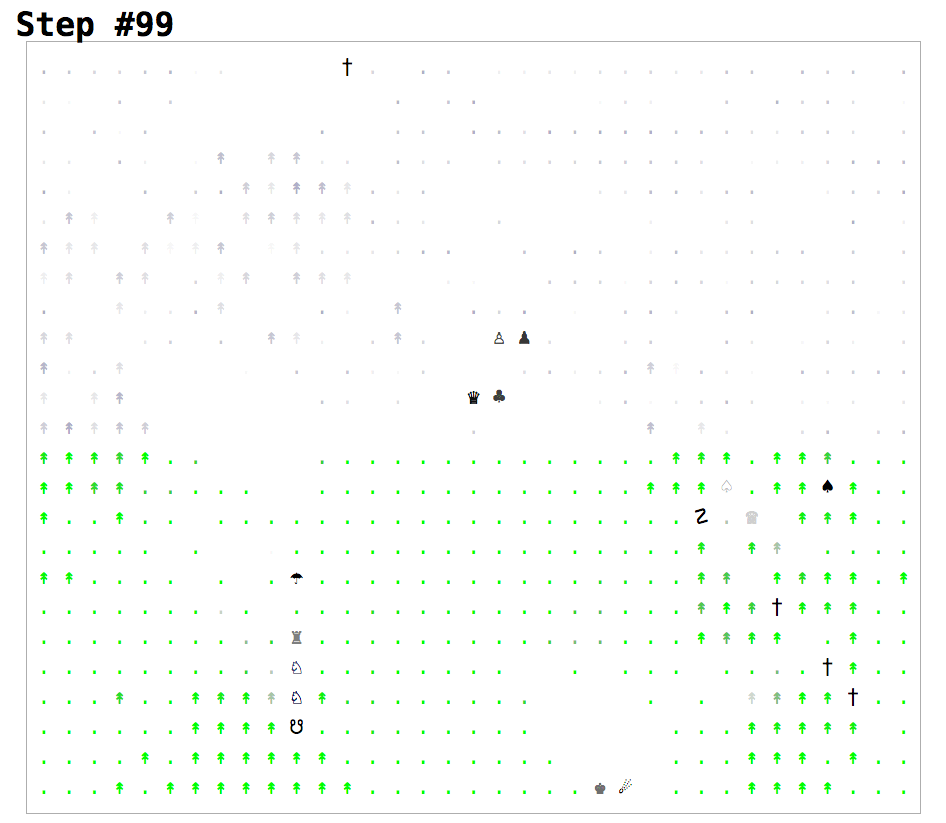
\includegraphics[width=0.7\linewidth]{screenshot_simulation.png}
\begin{captionbelow}{a screenshot of the running simulation}\end{captionbelow}
\end{figure}

According to the working hypothesis, cognition can extend to any characteristic related to survivability. This core characteristic, at the heart being an information theoretic definition, lends itself naturally to computer modeling. This affords a very convenient means of modeling via computer simulation. In contrast, a strictly biological view of cognition would rely upon the need for a simulation that had some biological validity. This would be very hard to implement and validate.

To explore the enhancement of cognition, various real-world enhancements of cognition were adapted in simplified form to the agent model: Among them being physical enhancements (e.g., reduced metabolism), perceptual enhancements (e.g., better vision, delayed environmental knowledge), and social enhancements (e.g., social pooling of knowledge, a system for making friends and enemies), and behavioral enhancements (e.g., individual greediness).

The envisioned and implemented simulation is a concrete, tangible and repeatable thought experiment. In a sense, it is a thought experiment for the computational age. In comparison to a classical thought experiment, the axioms and assumptions of the computerized thought experiment are not formally stated in explicit terms, but rather implicitly in the formal language of programming. Interestingly, there is a direct equivalence: Both approaches yield a comparable result, that is well-defined and graspable to the human mind, yet mechanic enough to lead to logical conclusions that might not have been envisioned in the first place.

Instead of trying to say something about objective reality the goal of this experiment is merely that of exploring definitions of the topic at hand in order to illustrate a more detailed view and understanding of cognition. In this respect, there may be biases induced by the experimenter's expectations, but they are unlikely to impugn the validity of the simulation, as the simulation can be interpreted as an investigation of the logical and functional integrity of these expectations by the experimenter.

The simulation, implemented for the experimental part of this thesis, is based on a reimplementation of the \textit{Sugar Scape} agent-based simulation. The code used is a freshly programmed interpretation of the original model, written in the \textit{Python} programming language in the dynamic programming environment of the \textit{IPython Notebook}. The main packages used in the implementation were \textit{IPython}, \textit{NumPy} and \textit{Cython}. IPython was used for its excellent qualities regarding scientific computing, its Notebook environment for its interactivity while programming, NumPy for its qualities in the lay-out and transformation of arrays, and Cython for computational optimization of slowly running code.

\section{The Flow of Time}

The underlying flow of the simulation is implemented in discrete time. This means that the global time of the agent-based simulation flows in single (discrete) steps. During each step, every agent is permitted to move once and the order in which the agents are moved is randomized for each step, so that no single agent has the advantage of always moving first, as this would compromise the model.

\section{The Model of the Suspending Environment}

The cells of the grid on which the agents move is constructed as an array of tiles. The tiles are an abstraction of an area of land. At the start of the simulation, every tile gets assigned a small random amount of sugar. Additionally, the grid is sprinkled with a certain number of randomly created little \textit{forests} of random higher quantities of sugar.

This initial state defines the maximum amount of sugar a cell can have. The maximum amount of sugar (\textit{max sugar}) a cell can have is important as it limits the regrowth of the sugar. When an agent passes over a cell, for each step of the simulation, the amount of sugar is harvested according to a certain ratio that is influenced by the agent's greed and its age.

\noindent
The environment is generated randomly with some `background sugar' \dots
\begin{minted}[autogobble]{python}
    grid = []
    for x in xrange(maxx):
        grid.append([])
        for y in xrange(maxy):
            sugar = max_sugar = randrange(1,10+1)
            grid[x].append(Tile(reverse_legend[sugar], 
                                (x,y), sugar, max_sugar))
\end{minted}
\dots and with some patches/`forests' of higher density:
\begin{minted}[autogobble]{python}
    grid = array(grid)
    for _ in xrange(randrange(5,10+1)):
        x, y = randrange(0,maxx), randrange(0,maxy)
        for r in xrange(randrange(2,5+1)):
            for side in radius(grid, (x,y), r):
                for tile in side:
                    sugar = randrange(10,30)
                    tile.sugar = tile.max_sugar = sugar
                    tile.orig_sym = reverse_legend[sugar]
\end{minted}

Although the max sugar a cell can have is a fixed trait of each tile, it is then modified during the running of the simulation. If a cell is overharvested, then it can loose carrying capacity through the decrease of the max sugar value. Whenever the growth of a cell reaches the amount of max sugar, then another metric, the amount of \textit{pollen} is increased until a certain threshold is reached. When this happens, the surrounding cells are \textit{pollinated} with an increase in max sugar, according to a random ratio of the pollen that was accumulated by the pollinating cell. This leads to fundamental changes in the simulated environment over time.

\begin{figure}[h]
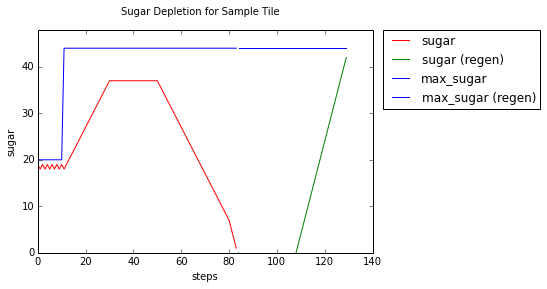
\includegraphics[width=0.7\linewidth]{growth.png}
\begin{captionbelow}{the red line shows the sugar being overharvested, with delayed regeneration}\end{captionbelow}
\end{figure}

The described mechanisms are of great importance to the model, as it, first of all, creates one of the aspects that create an ever-changing environment and, second, leads to the simulated reality in which the behavior of the agents actually shapes their suspending environment. 

The sugar can never become negative.

These changes in environment are made more dynamic through the implementation of four seasons and two hemispheres that have opposing seasons. The seasons lead to growth in the spring and summer and decay in the winter. They also directly influence the metabolism of the agents. Agents need to expend more energy to get through the winter and less in the spring and summer.

\noindent
The mechanisms by which the sugar grows and even sprouts (fundamentally changing the environment):
\begin{minted}[autogobble]{python}
        if growth > 0 and self.sugar + growth > self.max_sugar:
            self.pollen += growth * 2
        else:
            self.sugar += growth
            
        if self.pollen > self.max_sugar:
            surrounding = radius(grid, self.pos, 2)
            num_tiles = sum(len(side) for side in surrounding)
            for side in surrounding:
                for tile in side:
                    new_sugar = tile.max_sugar + self.pollen // num_tiles
                    if (abs(tile.max_sugar - new_sugar) > 
                            abs(self.max_sugar - new_sugar)):
                        tile.orig_sym = self.orig_sym                        
                    tile.max_sugar = new_sugar
            self.pollen = 0
\end{minted}

The following code snippets illustrates the mechanism by which the environment effects agents directly (sugar) and indirectly (metabolism):

\begin{itemize}
    \item season increases or decreases metabolism:
\end{itemize}
\begin{minted}[autogobble]{python}
        season = grid[self.pos].season
        metabolism_mult = {'summer': .75, 'winter': 1.25, 
                           'spring':  .5, 'autumn':    1}
        
        metabolism = (int(ceil(metabolism_mult[season] * 
                         self.metabolism * self.age / 250)))
\end{minted}
\begin{itemize}
    \item also, sesaon increases or decreases sugar growth rate
\end{itemize}
\begin{minted}[autogobble]{python}
        if self.delay:
            growth = 0
            self.delay -= 1            
        elif self.season == 'spring':
            growth = self.max_sugar//40
            if growth < 2:
                growth = 2
        elif self.season == 'summer': 
            growth = self.max_sugar//50 
            if growth < 1:
                growth = 1
        elif self.season == 'autumn':
            growth = 0
        elif self.season == 'winter':
            growth = -self.max_sugar//30
            self.pollen = 0
\end{minted}

\section{The Criticality of a Changing Environment to Cognition}
The aforementioned properties of the environments are of great importance to the simulation at hand. The changing environment creates a habitat were better cognition makes a large difference. The simpler the surrounding environment, the less complex the agent cognition has to be in order to still compete and survive well.

\section{Agent Aging}
To model the effects entropic forces have on organisms in the real world, the agents are programmed to age. Aging (number of steps) increases metabolism and over time this slowly but surely ends up hurting the agents. This happens up to a point were the agents can not support their metabolism anymore and die of hunger. 

\begin{itemize}
    \item metabolism starts slowing down at 250 steps, increasing linearly:
\end{itemize}
\begin{minted}[autogobble]{python}
        metabolism = (int(ceil(metabolism_mult[season] * 
                         self.metabolism * self.age / 250)))
\end{minted}

\section{Reproduction}

The agents give birth and growing population means more competition. Each agent that exceeds a certain amount of `wealth' can reproduce. Reproduction only happens with a certain likelihood, which is determined by a certain chance and a randomization function.

Children directly inherit characteristics from parents such as vision, greed, and cognition. They can have small, random mutations.
Children `cost' some wealth to give birth to: this can be viewed as birthing cost and/or as inheritance cost.

\noindent
The following code presents the reproduction mechanism:
\begin{minted}[autogobble]{python}
    def reproduce(self, step):
        child = Agent(name = "{}'s child".format(self.name),
              sym = self.orig_sym,
              metabolism = self.metabolism,
              wealth = self.wealth//4,
              vision = (clip(self.vision + randrange(-2,2),
                              0, 10)),
              greed = (clip(self.greed + randrange(-5,5),
                              0, 10)),
              cognition = (clip(self.cognition        
                              + randrange(-1,1), 0, 3)),
              pos = self.pos,
              birth_step = step,
              parent = self)            
        self.children.append(child)
        self.wealth -= self.wealth//4
        return child
\end{minted}

\subsection{Brood Care}
 Agents take care of their young, as they can't move for their first 100 steps; they will die unless they are fed. Only `adult' agents can eat, only `adult' agents can move; therefore, `children' agents must rely on parents to survive:
 
\begin{minted}[autogobble]{python}
        if self.age > 100:
            sugar = self.eat(metabolism, tile=grid[self.pos])

        if self.age > 100:
            self.move(dest, grid)
\end{minted}

\section{Friends, Enemies, Families, Competition and Sharing}

The agents are in direct competition and by default, all other agents are their enemies. In contrast, children and other family are generally considered friends.

Agents only share with their friends, which their families are part of by default. This models tribal affiliations as the `tribes' not only share among themselves, but also fight against other tribes, as everyone else is by default considered an enemy.
 
\noindent
The following code illustrates the process by which friends and enemies are created:
\begin{minted}[autogobble]{python}
        for other in other_agents:
            if (other is not self and
               other not in self.friends and
               other not in self.enemies):
                if (other.parent in self.friends or
                   other.parent is self or
                   self in other.children):
                    self.friends.add(other)
                elif other.parent in self.enemies:
                    self.enemies.add(other)
                else:
                    self.enemies.add(other)      
\end{minted}
\noindent
They share with agents nearby and fight agents nearby; they also use the presence or absence of an agent within their line-of-sight as a modifier for where to move:
\begin{minted}[autogobble]{python}
         for other in other_agents:
             if self is not other and other.alive:
                 ox, oy = other.pos
                 ovx, ovy = ox - xvmin, oy - yvmin
                 for r in (0,1,2):
                     ovxmin, ovxmax = (clip(ovx-r, vminx, vmaxx), 
                                       clip(ovx+r+1, vminx, vmaxx))
                     ovymin, ovymax = (clip(ovy-r, vminy, vmaxy),
                                       clip(ovy+r+1, vminy, vmaxy))

                     if other in self.enemies:
                         view[ovxmin:ovxmax, ovymin:ovymax]*=.95
                     elif other in self.friends:
                         view[ovxmin:ovxmax, ovymin:ovymax]*=1.05
\end{minted}
 
\section{Limited Information of the Agents Subjective Reality}
In order for the agents to act as individual entities within a subjective view of the world, their mental model of the world has to be created by sensory acquisition. This by nature leads to a limited information model of the surrounding world. In itself this would already be an interesting trait, but in this model the agents' subjective world is also influenced by their character traits. The mental model of the world is morphed according to individual traits, that the children inherit from their parents.

\noindent
Agents can only see and react to agents within their vision:
\begin{minted}[autogobble]{python}
            kdt = KDTree([agent.pos for agent in agents])
            other_agents = (agents[kdt.query_ball_point(
                               agent.pos,agent.vision)])
\end{minted}
They only make their decision on where to move based on information in their radius of sight:
\begin{minted}[autogobble]{python}
        # look around
        # vision-adjusted minima, maxima
        x, y = self.pos
        xvmin, xvmax = (clip(x-self.vision, minx, maxx),
                        clip(x+self.vision+1, minx, maxx))
        yvmin, yvmax = (clip(y-self.vision, miny, maxy),
                        clip(y+self.vision+1, miny, maxy))
\end{minted}
\noindent
And there is some inexactness to their model. Their view of the environment (which they use to decide how to move) is fuzzed to represent imperfect knowledge:
\begin{minted}[autogobble]{python}
        # fuzzing
        view *= 1 + ((.5 - random(view.shape)) / 50)
\end{minted}

\section{Reduced Cognition}
Some of the agents have a limited cognition: Their knowledge of the grid can be delayed by a couple of time-steps. According to the their `cognition value', the cognition is exponentially delayed:
At best they see the actual state of the world, then, with one step of lessened cognition, the state of the world delayed by 1 step or 4 steps or 9 steps or 16 steps...

\begin{minted}[autogobble]{python}
                density_grid = density_grids[agent.cognition ** 2]
\end{minted}

\section{Agent Character Traits}

The simulation is a mockup of how the environment has to shape certain characteristics of an agent in order to survive. Since it is very hard to program a simulation in a way that the agents evolve without intervention, another approach has been taken. The experiment takes on the role of a `god' and imposes certain characteristics, in order to see how they change the success or behavior of the agents. To have some knobs by which certain behaviors could be modified, agent character traits were implemented in a way that they could take on various discrete values that affect the agent's needs and view of the world.

\subsection{Greedy Parameter}

The greedy parameter assigns a certain amount of greediness to an agent that does not change over time and that will be inherited to its children. Therefore, the effect on a single agent can be evaluated, as well as the effect it has on many generations of an agent population and the growth or depletion of its relative sugar environment.

The greed of an agent is a multiplier on the amount an agent harvests each step. By this mechanism, greedy agents get wealthier more quickly, but they can also deplete their environment more easily. This leads to an interesting tension between the optimization for maximum wealth in the short term and the amount of wealth that can be extracted by a population over time.

\subsection{Seeking Novelty Parameter}
This parameter changes the agent's lust for novelty. The parameter encourages agents to move to cells that they have less frequently visited.

\chapter{Results}

\section{Core Differences to \textit{Sugar Scape}}
The model at hand is a variation on the \textit{Sugar Scape} model. What makes this model special, is:
\begin{description}
\item[First,] in this thesis' model, the environment is continuously changing. This differs from the original \textit{Sugar Scape} in that sugar does not only get depleted and grow back, but that it can actually sprout and overgrow or be permanently depleted. This leads to the interesting dynamic that over time the agent population influences how their environment develops, which in return will influence future agent generations' ability to extract wealth from the environment.
\item[Second,] the agents have a subjective reality that is unique not only in the part of the grid that they can see, but the individual relevant aspects of the surrounding world get integrated into a subjective \textit{Umwelt} of each grid. Technically, this is implemented by separate grids that vary according to different aspects of the surroundings. These morphed grids that can stand for enemy avoidance, brood care, or even signify the agents greed, are then all integrated into a unified and individual view of the world that agents maximize over in order to determine their next steps.
	\item[Third,] the state of the agent, whether it is parenting, barely surviving or something other, directly influences this subjective view of the world by the weighting of the multipliers for the integration of the different sub-grids that make up the mental model of the agent.
\end{description}
\clearpage
\section{Observations}
As part of the investigation, quantitative data was collected, but this data will not be presented in this section, as the experiment does not try to prove anything in particular. The experiment's purpose was merely as a reflection of the practical aspects of the working hypothesis and therefore the model was developed as a playful, interactive investigation, a computational thought experiment with the observer actively molding and supervising the creation of his own consistent simulated reality.

\noindent
The following will describe some key observations made during this time:

Goal oriented and social behaviors were the most successful survival strategies. These enhancements naturally adapted to increases in the complexity of the environment the agents were confronted with. The clear tendency was that the more complex the interactions in the model, the more value goal orientation and social behaviors actually created.

In this regard, what is especially important to the topic of the thesis, is that all changes internal to the agent, such as goal orientation, better vision or otherwise, can have a similarly enhancing effect on the survivability of the agent as the implementation of social behaviors.

What was especially interesting in regard to the social behaviors, is that the hardship single agents were confronted with, were largely compensated for by the other members of the `tribe'. This simple reality of the agent model nicely compares to the real world, as it describes a kind of social insurance through friendship and altruism.

\section{Questions Raised During the Observation}
\begin{description}
  \item[Transparency:] Is causality obvious in the simulation? Can it be asserted that a result is definitely caused by something?
  \item[Obviousness:] Are results obvious? Can one clearly say that some (more complex) behavior emerged?
  \item[Tractability:] Can one tractably model this? Is it possible for a single programmer to write the code to do this?
  \item[Complexity:] How much complexity does this code need to have to demonstrate results?
\end{description}

\section{Compexity --- Pros and Cons}
In the creation and running of the simulation it clearly showed that, from a single feature, we cannot see any emergent behavior beyond that feature. In order to see more emergent behaviors, more complexity needs to be introduced. Complexity comes from the interaction of features, but the more complexity one introduces, the more difficult it becomes to identify causal factors.

\section{General Observations and Thoughts}

The agent simulation is purely behavioral and is missing any element of `higher order choice': e.g. the agent can be directed to make choices as first order results of a given value system, but there is no emergent behavior resulting from an unbounded order/recursion/feedback of this mechanism. This dramatically simplifies the simulation, but limits the ability to see complex behaviors emerge. 

Nevertheless, it was possible to observe behaviors and causalities independent of this higher choice. The non-presence of the factor of higher order choices is particularly meaningful, because the manifestation of desired behaviors suggests that simple models (such as rational agent theory in economics) may in some cases be sufficiently complex to make real-world predictions.

\noindent
It could be observed that cognition in the agents is a combination of the following:
\begin{itemize}
  \item a changing environment with limited resources
  \item the presence of other agents competing for these resources
  \item a direct view of this environment (sensory-limited knowledge)
  \item a delay-function on knowledge of the system (cognition)
  \item a variety of agent states and characteristics (state = wealth, characteristic = greed, metabolism)
  \item a set of weighted value-functions (with agent-specific local, limited knowledge) that guide a decision based on the above
\end{itemize}

\chapter{Discussion}

Even though many of the observations where already discussed in-line in the results section, there are a few things to add and conclude:

It was possible to conclusively show differences in survivability relative to the factors designed to change agent cognition. The ease of pinpointing causal factors for these differences in survivability was supported by the simplicity of the model.

By modifying the behaviors and traits of two distinct groups of agents, it was possible to argue about certain advantages and disadvantages of cognitive traits. Having constructed these dichotomies, it was only necessary to construct simple systems to argue for the facts that the model suggests. This shows that one can create a universe that is much smaller than the infinite complexity of the real world and recreate some of the same dynamics that can be observed in the infinitely complex. The less complex the world is, the harder it gets to give a meaningful advantage by cognition. This leads to a situation where complexity and obviousness have to be balanced in order to ameliorate our insights into the complex world of social dynamics.

It is clear that some characteristics of complex behaviors in humans can sometimes be seen in the much smaller scale world of small organisms. However, there is an important field of investigation in determining precisely which simulated factors are necessary in the simplified environment to account for the real world phenomena under investigation.

Another interesting aspect of the simulation is that above certain (relatively low) level of cognition, the strength of an agent's cognition is very hard to differentiate ad hoc. It almost always needs multiple generations to determine if a seeming advantage in cognition actually translates into a long-term sustainably positive effect.

As it turns out, it is really hard to see what makes smartness or dumbness just from a life graph. The only way that we can truly say if a behavior leads to long term gains, is to see if the agent or group of agents can sustain itself/themselves at that level of life quality or whether the population collapses back in on itself as the newly created demand outstrips the available supplies.

Even though no absolute causality is implied with the simulation itself, it can be argued that it is a kind of constructive proof that demonstrates the plausibility of a given descriptive model of phenomena in the real world. Looking at the model as a kind of black box, one might see some of the same behaviors that you might get from a much more dynamic model or system. 

Epistemologically, it is hard to demonstrate whether the implemented experimental model actually maps to reality, because of the fact that these characteristics in reality are too complex to model transparently. Direct, physical, or non-representational modeling of these real world characteristics can suggest greater accuracy but modeling them risks loss of insight into the internal operation of the model which prevents identification of new causal factors. However, overly representational, symbolic, or abstract modeling offer a simplicity that affords greater understanding of these internal mechanisms but risks subjecting the model to the biases of its creator. Yet, at the crossroads of these two aspects there sits a window of insight into the aspects of highly interactive systems with their inherent dynamic and complexity.

\chapter{Conclusion}
Humanity, having reached a historical population high of 7 billion, is still not the most populous species on the planet. However, in most ecosystems, humans go beyond being just an apex predator to being the most dominant force of change in their ecosphere. By the accumulative effects of individual human actions, fundamental changes have occurred involving all the living systems in the ecosphere. The decimation of species, rain forests and the over saturation of the atmosphere with green-house gases are just two examples of the stark effects accumulated human action can have on the world.

Humans tend to feel that they are superior to other species by being more intelligent. But even if it is really humans having the most mental capacity, this can in no way negate the fact that almost all nutrition a human needs to live is composed of ecological matter and that the oxygen any human breathes is a product of plant metabolism. By not realizing what effect human collective action is having on its nourishing environment and, especially if not acting by that realization, humans, by fact of existing or ceasing to exist, will endanger their very own egoistic motives of personal survival and, only second to that, their personal fulfillment.

Anything that helps humans reach the collective as well as individual goal of self-sustainment, should, by terms of the working definition established in this thesis, be considered to be cognitive enhancement.

Concurrently, any discussion of specific techniques of CE, be it education or neuropharmacological enhancement, should therefore be morally judged in the framework that has been laid out in this thesis. Also, the term of cognitive enhancement should \underline{not} be used for pharmaceutics, whose effect is not established to be mostly beneficial to the treated. One class of drugs that are proven to have little to no side-effects is that of noo-tropics: It deserves the umbrella term of CE, yet not a single of the usual suspects (Ritalin, etc.) in the raging CE debate are in the class of noo-tropics.

On the other hand, the treatment of the healthy with potentially cognitive enhancing drugs should be de-taboo-ized in order to make room for a truly scientific quest for substances and other ways, whatever they might be, to enhance our life-quality and ultimately our survivability being suspended in the ecosystem of this planet.

\newpage
\bibliographystyle{apacite}
\setlength\bibsep{\parskip}
\bibliography{enhancing_cognition}{}
\null
\vfilneg
{\let\clearpage\relax\listoffigures}


\addchap{Appendix --- Simulation Source Code}


\addsec{Preamble}
\begin{minted}[autogobble]{python}
% matplotlib inline
from __future__ import unicode_literals, division
\end{minted}


\addsec{Tile Model}
\begin{minted}[autogobble]{python}
from numpy import array, clip, copysign
from numpy.random import normal
from math import ceil
from collections import deque
from itertools import repeat, chain, cycle

# this object represents a tile in the grid
class Tile(object):
    def __init__(self, sym, pos, sugar, max_sugar = 100):        
        self.orig_sym = sym
        self.max_sugar = max_sugar
        self.sugar = (0 if sugar < 0 
                      else max_sugar if 
                      sugar > max_sugar 
                      else sugar)
        self.pollen = 0
        self.pos = pos   
        self.delay = 0

        self.season, self.cycle = None, None
        
    def __repr__(self):
        return 'Tile(pos={s.pos}, sugar={s.sugar})'.format(s=self)


    @property
    def rgba(self):        
        a = self.sugar / self.max_sugar if self.max_sugar != 0 else 0
        r = int(255*a if self.max_sugar < 0 else 0)
        if self.season in ('spring', 'summer'):
            g, b = int(255*a if self.max_sugar > 0 else 0), 0
        elif self.season in ('autumn', 'winter'):
            g, b = 0, int(255*a if self.max_sugar > 0 else 0)
        else:
            g, b = 0, 0 
        return '{r},{g},{b},{a}'.format(r=r, g=g, b=b, a=a)
    

    @property
    def sym(self):
        return '<span style="color: \
                rgba({s.rgba})">{s.orig_sym}</span>'.format(s=self)
        
    def harvest(self, sugar=1):
        if self.sugar == 0:
            self.delay = int(clip(self.delay*2, 10, 100))
            # self.max_sugar -= 5
            return 0
        sugar = int(clip(sugar, 0, self.sugar))
        self.sugar -= sugar        
        return sugar

    def step(self, grid, num):
        
        if self.season is None:
            lenx, leny = grid.shape
            equator = leny // 2
            north_hemi = xrange(0, equator+1)
            longitude, latitude = self.pos
            if latitude in north_hemi:
                self.cycle = cycle(chain(
                    repeat('spring', 30),
                    repeat('summer', 20),
                    repeat('autumn', 30),
                    repeat('winter', 20), ))
            else:
                self.cycle = cycle(chain(
                    repeat('autumn', 30),
                    repeat('winter', 20), 
                    repeat('spring', 30),
                    repeat('summer', 20), ))
        
        self.season = next(self.cycle) # change the season
        
        if self.delay:
            growth = 0
            self.delay -= 1            
        elif self.season == 'spring':
            growth = self.max_sugar//40
            if growth < 2:
                growth = 2
                
        elif self.season == 'summer':
            growth = self.max_sugar//50 
            if growth < 1:
                growth = 1
                
        elif self.season == 'autumn':
            growth = 0
            
        elif self.season == 'winter':
            growth = -self.max_sugar//30
            self.pollen = 0
        
        # XXX: only handles positive sugar amounts (no poison)
        if growth > 0 and self.sugar + growth > self.max_sugar:
            self.pollen += growth * 2
        else:
            self.sugar += growth
            
        if self.pollen > self.max_sugar:
            surrounding = radius(grid, self.pos, 2)
            num_tiles = sum(len(side) for side in surrounding)
            for side in surrounding:
                for tile in side:
                    if (tile.max_sugar <= self.max_sugar and 
                       tile.max_sugar + self.pollen //
                       num_tiles >= self.max_sugar):
                        tile.orig_sym = self.orig_sym
                    tile.max_sugar += self.pollen // num_tiles
            self.pollen = 0

def make_grid(grid, legend, agents):
    grid = grid.strip()
    g = []
    a = {}
    for row in grid.split('\n'):
        if row.strip():
            g.append([])
            for col in row.strip():
                col = col.strip()
                if col:
                    pos = len(g[-1]), len(g)-1
                    if col in legend:
                        sym = col
                    elif col in agents:
                        a[col] = pos
                        sym = '.'
                    else:
                        sym = '.'
                    sugar = legend.get(sym, 0)
                    g[-1].append(Tile(sym, pos, sugar, max_sugar=sugar))
                
    return array(g).T, a
\end{minted}

\addsec{Radius \& Density Grid Functions}
\begin{minted}[autogobble]{python}
%load_ext cythonmagic

%%cython

from numpy import zeros_like, empty_like, zeros
from numpy import clip, array, sqrt

def distance(pos1, pos2):
    x1, y1 = pos1
    x2, y2 = pos2
    return sqrt((x1-x2)**2 + (y1-y2)**2)  

def manhattan_distance(pos1, pos2):
    x1, y1 = pos1
    x2, y2 = pos2
    return abs(x2 - x1) + abs(y2 - y1)


def radius(g, pos, r):
    if r == 0:
        return [g[pos]],
    
    x, y = pos
    
    minx, miny = 0, 0
    maxx, maxy = len(g) - 1, len(g[0]) - 1

    #xvmin, xvmax = clip(x-r, minx, maxx), clip(x+r, minx, maxx)
    #yvmin, yvmax = clip(y-r, miny, maxy), clip(y+r, miny, maxy)
    
    xvmin, xvmax = x-r, x+r
    yvmin, yvmax = y-r, y+r
    
    if xvmin < minx: xvmin = minx
    elif xvmin > maxx: xvmin = maxx
    
    if xvmax < minx: xvmax = minx
    elif xvmax > maxx: xvmax = maxx
        
    if yvmin < miny: yvmin = miny
    elif yvmin > maxy: yvmin = maxy
        
    if yvmax < miny: yvmax = miny
    elif yvmax > maxy: yvmax = maxy     

    top = g[xvmin:xvmax+1, yvmax]
    bot = g[xvmin:xvmax+1, yvmin]
    lef = g[xvmin, yvmin+1:yvmax]
    rgt = g[xvmax, yvmin+1:yvmax]
    
    return top, rgt, bot, lef

def density(g, agents=None):
    Tile = type(g[0,0])
    d = zeros_like(g)

    agent_loc = empty_like(g, dtype=object)
    for agent in agents if agents is not None else []:
        if not agent_loc[agent.pos]:
            agent_loc[agent.pos] = []
        agent_loc[agent.pos].append(agent)
        
    for x, col in enumerate(g):
        for y, row in enumerate(col):
            t = g[x,y]
            d[x, y] = Tile(t.sym, t.pos, t.sugar, t.max_sugar)
            
            for agent in agent_loc[x,y] or []:
                d[x, y].sugar -= agent.metabolism
                d[x, y].max_sugar -= agent.metabolism
                
            for r in [1, 2]:
                sides = radius(g, (x,y), r)
                sugar = sum(tile.sugar 
                             for side  in sides
                             for tile in side) // ((r+2)**2)
                
                agent_sides = radius(agent_loc, (x,y), r)
                metabolism = (sum(agent.metabolism 
                                   for side in agent_sides
                                   for group in side 
                                   for agent 
                                   in (group or [])) // (r**2))
                
                d[x, y].sugar += sugar - metabolism
                d[x, y].max_sugar += sugar - metabolism
            
            # fuzz these values
            d[x ,y].sugar = d[x ,y].sugar // 4 * 4
            d[x ,y].max_sugar = d[x ,y].max_sugar // 4 * 4

    return d
\end{minted}


\addsec{Agent Model}
\begin{minted}[autogobble]{python}
from __future__ import unicode_literals
from numpy import sign, ceil, clip, empty, argmax, zeros_like
from collections import deque, namedtuple
from numpy.random import random
from operator import attrgetter


Heartbeat = namedtuple('Heartbeat', 
                       'sugar max_sugar metabolism wealth season pos')

class Agent(object):
    def __init__(self, name, sym, metabolism, wealth, 
                 vision, greed, cognition, pos, parent=None):
        if wealth <= 0:
            raise ValueError('initial wealth must be > 0')
        
        self.name = name
        self.orig_sym = sym
        self.metabolism = metabolism
        self.init_wealth = self.wealth = wealth
        self.vision = vision
        self.greed = greed
        self.cognition = cognition
        self.init_pos = self.pos = pos
        
        self.messages = deque(['Was just born!'])
        self.record_message = lambda _: None #messages.append
        self.retrieve_message = lambda _: None #messages.pop
        self.vitals = []
        
        self.max_tiles = set()
        self.child_tiles = set()
        
        self.children = []
        self.parent = parent
        
        self.has_shared, self.has_fought, self.has_reproduced = 0, 0, 0
        
        self.visited = None
        
        self.friends = set()
        self.enemies = set()
       
    def __repr__(self):
        return unicode(self).encode('utf-8')
    
    # TODO: color code agents (based on wealth?)
    def __unicode__(self):
        return 'Agent({s.name}, {s.sym}, {s.metabolism}, {s.wealth}, \
                      {s.vision}, {s.pos})'.format(s=self)
    
    @property
    def sym(self):
        r = 255//3 * self.has_fought
        g = 255//3 * self.has_shared 
        b = 255//3 * self.has_reproduced 
        rgba = '{r},{g},{b},{a:.4f}'.format(r=r, g=g, b=b, 
                a=clip(self.wealth/self.init_wealth, 0, 1))
        return '<span style="color: rgba({rgba})">{sym}</span>'.format(
               rgba=rgba, sym=self.orig_sym) if self.alive else '†'
    
    @property
    def alive(self):
        return self.wealth >= 0
    
    @property
    def age(self):
        return sum(1 for hb in self.vitals if hb.wealth >= 0)
    
    def reproduce(self):
            child = Agent(name = "{}'s child".format(self.name),
                    sym = self.orig_sym,
                    metabolism = self.metabolism,
                    wealth = self.wealth//4,
                    vision = self.vision ,
                    greed = self.greed,
                    cognition = self.cognition,
                    pos = self.pos,
                    parent = self)            
            self.children.append(child)
            self.wealth -= self.wealth//4 

            return child
    
    def eat(self, metabolism, tile):
        if self.wealth < 10:
            hunger = 10
        else:
            hunger = ((self.metabolism / self.wealth) * 
                       self.init_wealth * self.greed)
        
        sugar = tile.harvest(int(metabolism*hunger))
        self.wealth += sugar

        return sugar
    
    def step(self, grid, density_grid, friend_grid, 
                    enemy_grid, other_agents, step):
        if self.has_shared: self.has_shared -= 1
        if self.has_fought: self.has_fought -= 1
        if self.has_reproduced: self.has_reproduced -= 1
        
        season = grid[self.pos].season
        metabolism_mult = {'summer': .75, 'winter': 1.25, 
                           'spring':  .5, 'autumn':    1}
        
        metabolism = int(ceil(metabolism_mult.get(season, 1) *
                     self.metabolism * self.age / 250))
        
        if not self.alive:
            self.vitals.append(Heartbeat(None, grid[self.pos].sugar, 
                            metabolism, self.wealth, season, self.pos))
            self.record_message('Rests in peace')
            return
        
        if (self.age > 150 and
            self.wealth > 50 and
            self.wealth > (self.init_wealth * .5) and
            (grid[self.pos] in self.max_tiles
                or
            grid[self.pos] in self.child_tiles)
            and choice([True] + [False]*9) ):
            child = self.reproduce()
            self.child_tiles.add(grid[self.pos])
            self.has_reproduced = 3
            child.has_reproduced = 3
                
        for r in (0,1,2):
            for side in radius(grid, self.pos, r):
                for tile in side:
                    if len(self.max_tiles) < 10:
                        self.max_tiles.add(tile)
                    else:
                        min_tile = min(self.max_tiles,
                                       key=lambda t: t.sugar)
                        if tile.sugar > min_tile.sugar:
                            self.max_tiles.remove(min_tile)
                            self.max_tiles.add(tile)
        
        for other in other_agents:
            if (other is not self and other not in 
               self.friends and other not in self.enemies):
                if other.parent in self.friends or other.parent is self:
                    self.friends.add(other)
                elif other.parent in self.enemies:
                    self.enemies.add(other)
                else:
                    self.enemies.add(other)
                    
        sugar = 0
        if not self.parent or self.age > 100:
            sugar = self.eat(metabolism, grid[self.pos])
        
        self.wealth -= metabolism
        
        ### determine movement ###
        
        minx, miny = 0, 0
        maxx, maxy = grid.shape
        
        # look around
        x, y = self.pos
        
        
        
        # vision-adjusted minima, maxima
        xvmin, xvmax = (clip(x-self.vision,   minx, maxx),
                        clip(x+self.vision+1, minx, maxx))
        yvmin, yvmax = (clip(y-self.vision,   miny, maxy), 
                        clip(y+self.vision+1, miny, maxy))
        
        view = empty((xvmax - xvmin, yvmax - yvmin), dtype=float)
        vminx, vminy = 0, 0
        vmaxx, vmaxy = view.shape
        
        for x in xrange(xvmin, xvmax):
            for y in xrange(yvmin, yvmax):
                view[x-xvmin, y-yvmin] = density_grid[x,y].sugar
        
        for other in other_agents:
            if self is not other:
                ox, oy = other.pos
                ovx, ovy = ox - xvmin, oy - yvmin

                for r in (0,1,2):
                    ovxmin, ovxmax = (clip(ovx-r, vminx, vmaxx), 
                                      clip(ovx+r+1, vminx, vmaxx))
                    ovymin, ovymax = (clip(ovy-r, vminy, vmaxy), 
                                      clip(ovy+r+1, vminy, vmaxy))

        sx, sy = self.pos
        svx, svy = sx - xvmin, sy - yvmin
                    
        for r in xrange(0,self.vision):
            svxmin, svxmax = (clip(svx-r, vminx, vmaxx), 
                              clip(svx+r+1, vminx, vmaxx))
            svymin, svymax = (clip(svy-r, vminy, vmaxy), 
                              clip(svy+r+1, vminy, vmaxy))
            view[svxmin:svxmax, svymin:svymax] *= (.95 **r) 
            
        view *= 1 + (.5 - random(view.shape) / 100)
        
        if self.visited is None:
            self.visited = zeros_like(grid, dtype=float) -1
        self.visited[self.pos] *= 2
        view += self.visited[xvmin:xvmax, yvmin:yvmax]
            
        t = argmax(view)
        
        tx, ty = t % vmaxx, t // vmaxx
        tx += xvmin
        ty += yvmin
        
        d = { ( 0, 0): '*',
              ( 0,-1): 'n', 
              ( 1,-1): 'ne', 
              ( 1, 0): 'e',
              (-1, 1): 'se',
              ( 0, 1): 's',
              ( 1, 1): 'sw',
              (-1, 0): 'w',
              (-1,-1): 'nw', }[sign(tx - x), sign(ty - y)]
        
        x, y = self.pos
        
        if not self.parent or self.age > 100:
             #if grid[self.pos].sugar < 5:   
            self.pos = x + sign(tx - x), y + sign(ty - y)
        
        for child in self.children:
            if (child.alive and 
                distance(self.pos, child.pos) > self.vision):
                cx, cy = child.pos
                self.pos = x + sign(cx - x), y + sign(cy - y)
                break


        self.pos = tuple(clip(self.pos, (minx,miny), (maxx-1,maxy-1))) 
            # clip to the grid

        self.vitals.append(Heartbeat(sugar, grid[self.pos].sugar, 
                        metabolism, self.wealth, season, self.pos))
        if self.wealth > 10:
            self.record_message(
                            'Fit as a Fiddle ({})'.format(self.wealth))
        elif self.wealth > 5:
            self.record_message('Healthy ({})'.format(self.wealth))
        elif self.wealth > 1:
            self.record_message('Hanging On ({})'.format(self.wealth))
\end{minted}

\addsec{Display Frame \& Simulate}
\begin{minted}[autogobble]{python}
from __future__ import unicode_literals
from IPython.display import display_html, clear_output
from scipy.spatial import cKDTree as KDTree
from time import sleep, time
from numpy import array
from numpy.random import shuffle
from collections import deque
from __builtin__ import any # pylab clobbered `any`

def display_frame(step, grid, agents, show_messages=True):
    template = '''
        <div style="font-family: monospace;">
            <h2>Step #{{step}}</h2>
            <div style="float: left; padding: .5em; \
            margin: 0 .5em 0 .5em; border: 1px solid #aeaeae;">
                <pre>{{grid}}</pre>
            </div>

            {message_panel}
        </div>
        '''.format(message_panel = '''
            <div style="margin: 0 1em 0 1em;">
                 <p>== messages ==</p>
                 <p>{messages}</p>
            </div>''' if show_messages else '' )

    agent_pos = {agent.pos: agent for agent in agents}
    
    output = []
    for y, row in enumerate(grid.T):
        output.append([])
        for x, col in enumerate(row):
            agent = agent_pos.get((x,y))
            if agent is not None:
                output[-1].append(agent.sym)
            else:
                output[-1].append(col.sym)
    
    messages = []
    if show_messages:
        for agent in agents:
            while agent.messages:
                messages.append('{}: {}'.format(agent.orig_sym,
                                           agent.messages.popleft()))
    
    return template.format(step=step,
                           grid='\n'.join(' '.join(row) 
                                          for row in output), 
                           states='', 
                           messages='</p><p>'.join(messages))

def simulate(grid, agents, steps=100, stop_early=True):
    density_grid = enemy_grid = friend_grid = density(grid, agents)
    density_grids = deque([(enemy_grid, friend_grid,
                            density_grid)] * 10)
    
    dead_agents = {}
    agents = array(agents) # use numpy array for added convenience
    
    for step in xrange(steps):
        start_time = time()
        
        for col in grid:
            for tile in col:
                tile.step(grid, step)
    
        density_grid = enemy_grid = friend_grid = density(grid, agents)
        density_grids.appendleft((enemy_grid, friend_grid, density_grid))        
        
        # keep only 5 entries; discard the rest
        while len(density_grids) > 16:
            density_grids.pop()
        
        if len(agents):
            shuffle(agents)
                
            kdt = KDTree([agent.pos for agent in agents])

            for agent in agents:
                density_grid, enemy_grid, friend_grid = ( 
                    density_grids[agent.cognition ** 2] )

                other_agents = ( agents[kdt.query_ball_point(agent.pos, 
                agent.vision)]
                
                agent.step(grid, density_grid, friend_grid, 
                           enemy_grid, other_agents, step)

            for agent in agents:
                if not agent.alive:
                    if agent not in dead_agents:
                        dead_agents[agent] = 0
                    dead_agents[agent] += 1

            agents = array([
                agent for agent in         
                set(agents) | set(child for agent in agents 
                                  for child in agent.children)
                if dead_agents.get(agent,0) < 25
            ])
        
        clear_output(wait=True)
        display_html(display_frame(step, grid, agents, False), raw=True)
        
        if stop_early and not any(agent.alive for agent in agents):
            return step+1

        elapsed = time() - start_time
        if .1 > elapsed:
            sleep(.1 - elapsed)
    
    return step+1
    
from numpy import array
from numpy.random import randint as randrange

class nearestdict(dict):
    def __missing__(self, key):
        new_key = min(self, key=lambda k: abs(k-key))
        return self[new_key]

def random_grid(maxx, maxy, legend):
    reverse_legend = nearestdict({v:k for k,v in legend.items()})
    
    grid = []
    for x in xrange(maxx):
        grid.append([])
        for y in xrange(maxy):
            sugar = max_sugar = randrange(1,10+1)
            grid[x].append(Tile(reverse_legend[sugar], 
                           (x,y), sugar, max_sugar))
    
    grid = array(grid)
    
    for _ in xrange(randrange(5,10+1)):
        x, y = randrange(0,maxx), randrange(0,maxy)
        for r in xrange(randrange(2,5+1)):
            for side in radius(grid, (x,y), r):
                for tile in side:
                    sugar = randrange(10,30)
                    tile.sugar = tile.max_sugar = sugar
                    tile.orig_sym = reverse_legend[sugar]
    
    return grid    
\end{minted}
\newpage

\addsec{Simulation Inputs \& Run}
\begin{minted}[autogobble]{python}
from itertools import count
from collections import defaultdict
counter = defaultdict(count().next)

def all_agents(agents):
    for agent in agents:
        yield agent
        for child in all_agents(agent.children):
            yield child
            
    
def print_agents(agents):
    row = ('{id:^3} {sym:^5} {age:^5} {children:^5} {name:<20} ' 
           '{init:^4}/{wealth:^5} {greed:^6} {metabolism:^6} '
           '{vision:^7} {cognition:^5} {pos:^10} {fe:^2}')

    print row.format(id='id', sym='sym', age='age', children='chd', 
                     name='name', metabolism='metab', init='init', 
                     wealth='wealth', vision='vision', greed='greed', 
                     cognition='cogn', pos='pos', fe='fe')

    for agent in all_agents(agents.values()):
        print row.format(id=counter[agent],
                         sym=agent.orig_sym, 
                         age=agent.age,
                         children=len(agent.children),
                         name=(agent.name[:15] + 
                               ('...' if len(agent.name) > 15 else ''),
                         metabolism=agent.metabolism,
                         init=agent.init_wealth,
                         wealth=agent.wealth,
                         vision=agent.vision,
                         greed=agent.greed,
                         cognition=agent.cognition,
                         pos='({p[0]:2d}, {p[1]:2d})'.format(p=agent.pos),
                         fe='{}/{}'.format(
                            ''.join(x.orig_sym for x in agent.friends),
                            ''.join(x.orig_sym for x in agent.enemies)) )

from __future__ import unicode_literals
from random import choice, randrange

agent_symbols = [ ... ]

grid, agent_pos = random_grid(35, 25, {'.': 0, '↟': 20}), {}

def random_pos(grid):
    x = randrange(0, len(grid))
    y = randrange(0, len(grid[0]))
    return x, y

agents = {}
for sym in agent_symbols:
    agents[sym] = Agent('', sym, metabolism = 1,   #choice([1,2,3]),                                  
                                 wealth     = 100, #randrange(50,100), 
                                 vision     = 10,  #randrange(1,10),
                                 greed      = 5,   #choice([1,2,3,4,5]),
                                 cognition  = 0,   #choice([0,1,2,3]),
                                 
print_agents(agents)
\end{minted}

\addsec{Simulate}
\begin{minted}[autogobble]{python}
% time simulate(grid, agents.values(), steps=100, stop_early=False)

print_agents(agents)
\end{minted}

\blankpage
\blankpage
\end{document}
